% !TeX spellcheck = en_US
\documentclass[french]{yLectureNote}

\title{Outils Mathématiques}
\subtitle{Analyse dimensionnelle}
\author{Paulhenry Saux}
\date{\today}
\yLanguage{Français}

\professor{S.Deheuvels}%sebastien.deveuhels.irap.omp.eu

\usepackage{graphicx}%----pour mettre des images
\usepackage[utf8]{inputenc}%---encodage
\usepackage{geometry}%---pour modifier les tailles et mettre a4paper
%\usepackage{awesomebox}%---pour les boites d'exercices, de pbq et de croquis ---d\'esactiv\'e pour les TP de PC
\usepackage{tikz}%---pour deiffner + d\'ependance de chemfig
\usepackage{tkz-tab}
\usepackage{chemfig}%---pour deiffner formules chimiques
\usepackage{chemformula}%---pour les formules chimiques en \'equation : \ch{...}
\usepackage{tabularx}%---pour dimensionner automatiquement les tableaux avec variable X
\usepackage{awesomebox}%---Pour les boites info, danger et autres
\usepackage{menukeys}%---Pour deiffner les touches de Calculatrice
\usepackage{fancyhdr}%---pour les en-t\^ete personnalis\'ees
\usepackage{blindtext}%---pour les liens
\usepackage{hyperref}%---pour les liens (\`a mettre en dernier)
\usepackage{caption}%---pour la francisation de la l\'egende table vers Tableau
\usepackage{pifont}
\usepackage{array}%---pour les tableaux
\usepackage{lipsum}
\usepackage{yFlatTable}
\usepackage{multicol}
\newcommand{\Lim}[1]{\lim\limits_{\substack{#1}}\:}
\renewcommand{\vec}{\overrightarrow}
\newcommand{\norm}[1]{||\overrightarrow{#1}||}
\begin{document}
\setcounter{chapter}{3}
	\chapter{Vecteurs de l'espace}
	\section{Opérations sur les vecteurs}
	\subsection{Produit scalaire}
	\begin{theorem}[Définition du produit scalaire]
\begin{flalign*}
\vec{A}\cdot \vec{B} &= x_1x_2+y_1y_2+z_1z_2\\
&= \norm{A}\times \norm{B} \times \cos(\widehat{\vec{A},\vec{B}})
\end{flalign*}
\end{theorem}
	\subsection{Produit vectoriel}
	\begin{theorem}[Définition]
Le produit vaut $\vec{u}\wedge \vec{v}=\begin{pmatrix}
u_yv_z-u_zv_y\\
u_zv_x-u_xv_z\\
u_xv_y-u_yv_x
\end{pmatrix}$
\end{theorem}
\begin{theorem}[Norme]
La norme de $\vec{u}\wedge \vec{v}$ vaut $\norm{u}\times\norm{v}\times|\sin(\widehat{\vec{u},\vec{v}})|$. Cependant, on peut aussi la calculer avec la méthode classique en connaissant les composantes ($\sqrt{x^2+y^2+z^2}$).
\end{theorem}
\section{Rotation d'une base orthonormée}
On considère le schéma suivant :

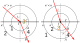
\includegraphics[scale=0.5]{fig1}

Alors, on peut exprimer les vecteurs $\vec{e_x}$ et $\vec{e_y}$ dans la base  $\vec{e_x'}$ et $\vec{e_y'}$ :
\[
\vec{e_x} = \cos (\alpha ) \vec{e_x'} -\sin(\alpha) \vec{e_y'}\\
\vec{e_y} = \sin( \alpha)  \vec{e_x'} +\cos(\alpha) \vec{e_y'}\\
\]

De la m\^eme façon, on peut exprimer les vecteurs $\vec{e_x'}$ et $\vec{e_y'}$ dans la base  $\vec{e_x}$ et $\vec{e_y}$ :
\[
\vec{e_x'} = \cos (\alpha ) \vec{e_x} +\sin(\alpha) \vec{e_y}\\
\vec{e_y'} = -\sin( \alpha)  \vec{e_x} +\cos(\alpha) \vec{e_y}\\
\]

On veut maintenant exprimer les composantes de $M$ dans le repère $R'$ en fonction des composantes de $M$ dans $R$ en projetant $x'$ et $y'$ dans le repère $R$ (projections rouges) :

\[
x' = \cos (\alpha ) x +\sin(\alpha) y\\
y' = -\sin( \alpha)  x +\cos(\alpha) y\\
\]
	\section{Méthode}
\subsection{Déterminer un vecteur directeur de m\^eme direction qu'un autre vecteur}
On veut déterminer le vecteur unitaire $\vec{u}$, de m\^eme direction que $\vec{AB}$. Pour trouver $\vec{u}$, il faut diviser les composante de $\vec{AB}$ par $\norm{AB}$ :
\[\vec{u} = \frac{\vec{AB}}{\norm{AB}}\]
\subsection{Utiliser le projeté orthogonal avec le produit scalaire}
Soit $\vec{AH}$, le projeté orthogonal de $\vec{AC}$ sur $\vec{AB}$.

Alors :
\begin{flalign*}
\vec{AB}\cdot \vec{AC} &= \norm{AB}\times \norm{AC}\cos(\alpha)\\
&= \frac{\cos (\alpha)}{\cos (\alpha)} \norm{AB}\norm{AC}\cos(\alpha)\\
&= \frac{\norm{AH}}{\cos (\alpha)} \norm{AB}\cos(\alpha)\\
&= \norm{AH}\times \norm{AB}\\
\end{flalign*}
\subsection{Exprimer 2 vecteurs de m\^eme direction l'un en fonction de l'autre}
Soit $\vec{AC}$ et $\vec{AB}$ deux vecteurs. On cherche $x$ dans $\vec{AC} = x \vec{AB}$ Donc $x = \frac{\norm{AC}}{\norm{AB}}$.
\subsection{Déterminer la valeur de l'angle entre 2 vecteurs avec le produit vectoriel}
En connaissant les coordonnées des 2 vecteurs u et v, on peut trouver leur produit vectoriel, ici noté $\vec{w}$.

On peut calculer la norme avec la formule $\sqrt{x^2+y^2+z^2}$

Le sinus de l'angle recherché vaut alors : \[\frac{\norm{w}}{\norm{u}\times\norm{v}}\]

En faisant le rapport, on trouve le sinus de l'angle, puis en appliquant $\sin^{-1}$ au rapport, l'angle, noté $\alpha$. Cependant, la valeur de $\alpha$ peut aussi \^etre : $\pi-\alpha, -\alpha, \alpha-\pi$.
\section{Formules trigonométriques}
\subsection{Équivalences}
\begin{itemize}
 \item $\cos(-a) = \cos (a)$
 \item $\cos(\pi-a) = - \cos(a)$
 \item $\cos(\frac{\pi}{2}-a) = \sin (a)$
 \item $\sin(-a) = - \sin(a)$
 \item $\sin(\pi-a) = \sin(a)$
 \item $\sin(\frac{\pi}{2}-a) = \cos(a)$
\end{itemize}
\subsection{Sommes}
\begin{itemize}
 \item $\cos(a+b) = \cos(a)\cos(b) - \sin(a)\sin(b)$
 \item $\cos (a-b) = \cos(a)\cos(b) + \sin(a)\sin(b)$
 \item $\cos(2a) = \cos^2(a)-\sin^2(a) = 2\cos(a)-1=1-2\sin(a)$
 \item $\sin(a+b) = \sin(a)\cos(b)+\cos(a)\sin(b)$
 \item $\sin(a-b) = \sin(a)\cos(b)-\cos(a)\sin(b)$
 \item $\sin(2a) = 2\sin(a)\cos(a)$
\end{itemize}
\subsection{Linéarisation}
\begin{itemize}
 \item $\cos(a)\cos(b) = \frac{1}{2}(\cos(a+b)+\cos(a-b))$
 \item $\sin(a)\sin(b) = \frac{1}{2}(\cos(a-b)-\cos(a+b))$
 \item $\sin(a)\cos(b) =  \frac{1}{2}(\sin(a+b)+\sin(a-b))$
\end{itemize}


\end{document}

